\subsection{Database}
MySQL was selected as database service technology.

ERD schematic is presented at the figure \ref{fig:database_erd_schematic}.
\begin{figure}[h]
    \centering
    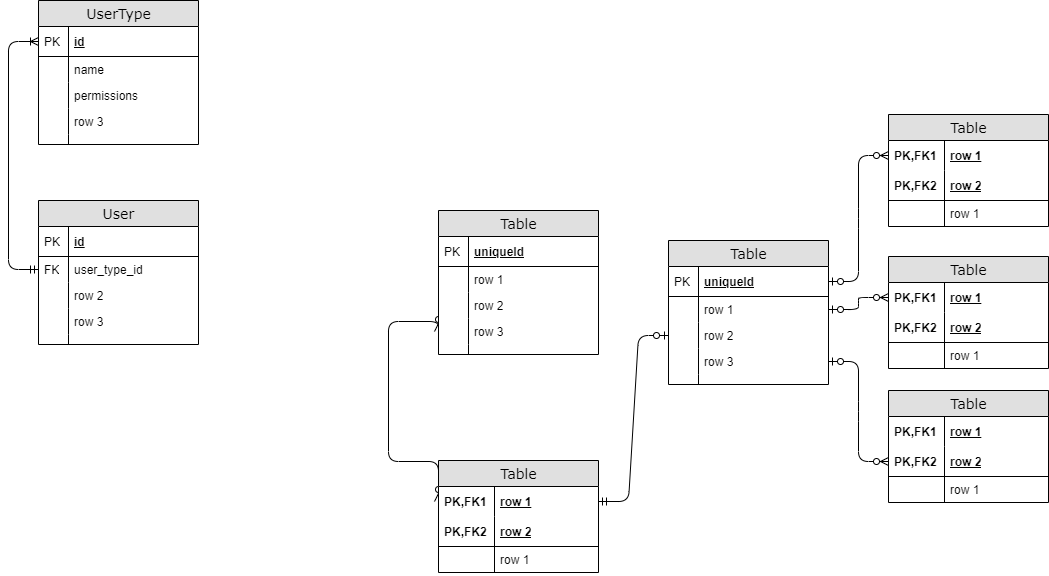
\includegraphics[width=\textwidth]{Include/Resources/Database/Project/databse_ERD_diagram.png}
    \caption{ERD schematic diagram}
    \label{fig:database_erd_schematic}
\end{figure}

\textit{UserType} table should be prepared before system deployment. Data from this table will be not available to change from the system.

\textit{User} table contains user data. Each of users in the system has separated entry. User type  is defined by userTypeId that reefers to the \textit{UserType} table.

\textit{UserToken} table 

\textit{BorrowedPeriod}  table contains information about how long book can be borrowed by user.

\textit{BorrowedPlace} contains the name of place where book can be read.
